\documentclass[aspectratio=169]{beamer}

% --- THEME SETUP ---
\usetheme{Madrid}
% \usecolortheme{beaver} % Red/Grey theme for "Top Secret" vibe
\setbeamertemplate{navigation symbols}{} % Hide navigation commands (icons)

% --- CUSTOM WHITE BANNER LOGO SETUP ---
\setbeamercolor{frametitle}{bg=white, fg=blue!70!black}
\setbeamertemplate{frametitle}{%
    \vspace{0.2cm}
    \begin{beamercolorbox}[wd=\paperwidth, ht=0.7cm, dp=0.2cm]{frametitle}
        \hspace*{0.5cm}\usebeamerfont{frametitle}\insertframetitle\hfill
        \raisebox{-0.3cm}{\includegraphics[height=1cm]{logo_univ_bdx.png}}\hspace*{0.5cm}
    \end{beamercolorbox}%
    \begin{tikzpicture}[remember picture,overlay]
        \draw[blue!70!black, thick] (current page.north west) ++(0,-1.3cm) -- ++(\paperwidth,0);
    \end{tikzpicture}
}

% --- PACKAGES ---
\usepackage[utf8]{inputenc}     
\usepackage[T1]{fontenc}
\usepackage{booktabs}
\usepackage{amsmath, amssymb}
\usepackage{tikz}
\usetikzlibrary{shapes.geometric, arrows.meta, positioning, calc}
\usepackage{pgfpages} % For speaker notes

% --- SPEAKER NOTES CONFIG ---
% Enable dual screen: Slides on Left, Notes on Right
\setbeameroption{show notes on second screen=right}
\setbeamertemplate{note page}[plain]

% --- LOGO CONFIG (MOVED TO FRAMETITLE) ---

% --- METADATA ---
\title{Operation Rubicon}
\subtitle{Analyse Cryptographique de la Vulnérabilité Minerva}
\author{Arnaud Gomes}
\institute{Université de Bordeaux}
\date{\today}

\begin{document}

% ==============================================================================
% 1. TITLE
% ==============================================================================
\begin{frame}
    \titlepage
    \note{
        Bonjour à tous. Aujourd'hui je vais vous parler de l'une des plus grandes affaires d'espionnage du 20ème siècle : l'Opération Rubicon.
        
        Pendant près de 50 ans, les agences de renseignement américaine (CIA) et ouest-allemande (BND) ont secrètement possédé la société suisse Crypto AG, qui était alors le leader mondial incontesté de la vente d'équipements de chiffrement et de sécurité des télécommunications pour les diplomates et tous les gouvernements.
        
        L'histoire que je vais vous raconter aujourd'hui montre que la vulnérabilité technique au sein de ces machines n'était pas une simple erreur de code. C'était une véritable porte dérobée (backdoor) mathématique, créée dès le départ pour écouter les communications du monde entier.
    }
\end{frame}

% ==============================================================================
% 2. CONTEXT (MULTIPLE SLIDES)
% ==============================================================================
\section{Contexte Géopolitique}

\begin{frame}{Le Contexte : Le Partenariat CIA / BND}
    \begin{columns}
        \column{0.4\textwidth}
        \textbf{L'Opération Rubicon (Thesaurus)}\\
        \vspace{0.3cm}
        \begin{itemize}
            \item Accord secret signé en 1970.
            \item Achat de Crypto AG via des sociétés écrans au Liechtenstein.
            \item Partage à 50/50 des bénéfices... et des interceptions diplomatiques.
        \end{itemize}

        \column{0.6\textwidth}
        \begin{center}
            \resizebox{\linewidth}{!}{
            \begin{tikzpicture}
                \node[draw=black, fill=red!10, text width=2.8cm, align=center, rounded corners] (cia) at (0,2.5) {
                    \includegraphics[height=1cm]{images/cia_seal.png}\\
                    \vspace{0.1cm}
                    \textbf{NSA / CIA}
                };
                \node[draw=black, fill=gray!20, text width=2.8cm, align=center, rounded corners] (bnd) at (0,-2.5) {
                    \includegraphics[height=1cm]{images/bnd_hq.jpg}\\
                    \vspace{0.1cm}
                    \textbf{ZFA / BND}
                };
                \node[draw=black, fill=blue!10, text width=3.2cm, align=center, rounded corners] (cag) at (6.5,0) {
                    \includegraphics[height=1cm]{images/crypto_ag_logo.png}\\
                    \vspace{0.1cm}
                    \textbf{Crypto AG} \\ 
                    \textit{Zoug, Suisse}
                };

                \draw[-{Latex[length=3mm]}, thick] (cia) to[out=0, in=120] node[above, sloped, midway, font=\footnotesize] {Cahier des charges} (cag);
                \draw[-{Latex[length=3mm]}, thick] (bnd) to[out=0, in=240] node[below, sloped, midway, font=\footnotesize] {Ingénierie} (cag);
                \draw[{Latex[length=3mm]}-, dashed, thick, red] (cia) to[out=-20, in=160] node[below, sloped, midway, font=\footnotesize] {Renseignements} (cag);
            \end{tikzpicture}
            }
        \end{center}
    \end{columns}

    \note{
        Pour bien comprendre la portée de cette attaque, je vais d'abord planter le décor. Tout commence en 1970, en pleine Guerre Froide. La CIA américaine et le BND d'Allemagne de l'Ouest signent un accord secret, nom de code Thesaurus, baptisé par la suite Rubicon.
        
        Ils rachètent secrètement la société Crypto AG, basée à Zoug en Suisse, en utilisant un montage financier très complexe de sociétés écrans. 
        
        L'objectif de cette entité est double : d'une part les deux agences se partagent les énormes bénéfices commerciaux, environ 50/50. Mais surtout, je tenais à insister, la NSA et la ZFA (l'agence ouest-allemande) imposent désormais les algorithmes de chiffrement qui seront implantés dans les machines. Ils contrôlent la chaîne de production.
    }
\end{frame}

\begin{frame}{Le Contexte : "Trusted" Hardware}
    \begin{columns}
        \column{0.5\textwidth}
        \begin{alertblock}{Le Couvert de la Neutralité Suisse}
            Leader mondial du chiffrement matériel (ex: HC-520, HC-570).
            Vendu à +120 pays sous couvert de stricte neutralité.
        \end{alertblock}

        \vspace{0.2cm}
        \textbf{Le Mécanisme Commercial :}
        \begin{itemize}
            \item \textbf{Machines Dédiées :} Boîtiers électromécaniques lourds.
            \item \textbf{Boîte Noire :} Algorithmes propriétaires hardware non-documentés ("Security by Obscurity").
            \item \textbf{Légitimité :} Promesse de sécurité mathématique par Boris Hagelin.
        \end{itemize}

        \column{0.5\textwidth}
        \begin{center}
            \includegraphics[height=3.5cm]{images/hagelin.jpg}\\
            \vspace{0.1cm}
            \tiny \textit{Une machine de type Hagelin CX-52.}
        \end{center}
    \end{columns}

    \note{
        Pourquoi le monde entier a-t-il acheté ces machines ? D'abord, à cause de la Suisse. Crypto AG bénéficiait de l'aura de neutralité politique, ce qui en faisait le fournisseur idéal.
        
        Ensuite, le produit était matériel ("hardware"). Comme vous le voyez ici à droite avec les machines inventées par Boris Hagelin, il s'agissait de blocs lourds, considérés inviolables physiquement.
        Les algorithmes de la série Cryptomatic (HC-500) étaient gravés dans le silicium : aucune spécification ou documentation mathématique n'était fournie. C'est le principe même de la "Security by Obscurity", un concept très dangereux en cryptographie.
    }
\end{frame}

\begin{frame}{Le Contexte : Les Deux Versions (A et B)}
    \begin{columns}
        \column{0.5\textwidth}
        \textbf{Version A : "Alliés"}
        \begin{itemize}
            \item États-Unis, Royaume-Uni, OTAN.
            \item Machines totalement sécurisées.
            \item Algorithme robuste non-compromis.
        \end{itemize}

        \column{0.5\textwidth}
        \textbf{Version B : "Le Reste du Monde"}
        \begin{itemize}
            \item Iran, Libye, Argentine, Inde, Vatican...
            \item Machines comportant la faille \textit{Minerva}.
            \item Messages lisibles en temps réel par NSA/BND.
        \end{itemize}
    \end{columns}
    
    \vspace{0.8cm}
    \begin{center}
        \textit{Même les ingénieurs et commerciaux de Crypto AG (ex: Hans Bühler en Iran) ignoraient manipuler des versions truquées.}
    \end{center}

    \note{
        Ce que les pays clients ignoraient évidemment, c'est que l'usine de Zoug produisait deux versions de la même machine en modifiant juste l'algorithme interne.
        
        La Version A, sécurisée organiquement, était vendue aux pays alliés de l'OTAN, comme le Royaume-Uni ou les Etats-Unis.
        La Version B était destinée au reste du monde : l'Iran, la Libye de Kadhafi, l'Argentine de la junte militaire, l'Inde... Ces machines contenaient la faille Minerva, permettant aux espions de lire les câbles diplomatiques en clair ou presque.
        
        J'ai trouvé fascinant de voir que le degré de secret était tel que même les ingénieurs concepteurs de chez Crypto AG ignoraient qu'ils vendaient des boîtes truquées. Seule une micro-cellule d'ingénieurs mathématiciens concevait la faille pour la NSA !
    }
\end{frame}

% ==============================================================================
% 2.5 HISTORICAL IMPACT SLIDES
% ==============================================================================

\begin{frame}{L'Impact Historique : Exploitation des failles}
    \textbf{Cas n°1 : La Guerre des Malouines (1982)}

    \vspace{0.3cm}
    \begin{itemize}
        \item \textbf{Le Contexte :} Conflit armé entre le Royaume-Uni (Fournisseur "Version A") et l'Argentine (Client Crypto AG "Version B").
        \item \textbf{L'Exploitation :} La junte militaire argentine chiffrait l'intégralité de ses communications navales tactiques avec des machines de la série Hagelin CX-52 / HC-500.
        \item \textbf{Résultat Opérationnel :} La NSA déchiffre les positions navales argentines en temps réel et transmet l'ordre de bataille exact à Londres.
    \end{itemize}

    \vspace{0.5cm}
    \begin{columns}
        \column{0.8\textwidth}
        \begin{alertblock}{La trahison diplomatique parfaite}
            L'Argentine, pensant son canal diplomatique sécurisé, négociait publiquement aux Nations-Unies tout en planifiant des frappes. Margaret Thatcher lisait les télégrammes avant même le président argentin.
        \end{alertblock}
    \end{columns}

    \note{
        Pour bien comprendre comment ce niveau d'espionnage mathématique se traduit sur le terrain, je propose deux exemples historiques majeurs. D'abord, la Guerre des Malouines en 1982.
        
        Lorsque l'Argentine envahit les îles, elle était totalement confiante dans ses communications chiffrées par ses machines Hagelin qu'elle jugeait ultra-modernes. L'erreur fut fatale. Le Royaume-Uni, pays ami des États-Unis et faisant partie de l'OTAN (donc utilisateur de la machine pure Version A), bénéficiait des écoutes totales.
        
        Grâce à la faille Minerva, la NSA craquait en temps réel les communications navales et diplomatiques argentines. Elle transmettait la position des sous-marins et des frégates au commandement de Margaret Thatcher. Dans le monde des agences, on raconte que Londres lisait les plans de la junte militaire plus rapidement que les propres généraux argentins.
    }
\end{frame}

\begin{frame}{L'Impact Historique : L'Iran et la Libye}
    \textbf{Cas n°2 : Espionnage étatique et Anti-terrorisme (Années 70-80)}

    \vspace{0.3cm}
    \begin{columns}
        \column{0.5\textwidth}
        \textbf{Crise des otages en Iran (1979)}
        \begin{itemize}
            \item Crise diplomatique : 52 américains retenus à Téhéran.
            \item Jimmy Carter (USA) observe la diplomatie ennemie en temps réel via l'interception des HC-500 iraniennes.
        \end{itemize}

        \column{0.5\textwidth}
        \textbf{Attentat "La Belle" Berlin (1986)}
        \begin{itemize}
            \item Ronald Reagan accuse Mouammar Kadhafi de l'attentat de Berlin-Ouest.
            \item Preuve formelle : Les télégrammes de "félicitations" libyens chiffrés par Crypto AG explosent silencieusement dans les serveurs de la NSA.
        \end{itemize}
    \end{columns}

    \vspace{0.6cm}
    \textit{Conséquence globale : Durant toute la Guerre Froide, la CIA a écouté plus de 120 pays sans la moindre résistance topologique.}

    \note{
        Je voudrais également aborder le Moyen-Orient. Lors de la Révolution Iranienne de 1979 et de la crise des otages, le régime islamiste utilise massivement les HC-500 "Version B" léguées par le Shah d'Iran. Le président américain Jimmy Carter déchiffre jour par jour les discussions internes du gouvernement de l'Ayatollah Khomeini... alors même que ceux-ci négocient contre lui !
        
        Plus tard, en 1986, lors de la bombe posée dans la discothèque berlinoise "La Belle", le président Ronald Reagan ordonne le bombardement de la Libye. Pour justifier cette frappe, l'administration américaine évoque des "preuves absolues". Ces preuves irréfutables s'avèrent être les câbles libyens chiffrés (des "Félicitations pour Berlin" envoyées de Tripoli) déchiffrés en quelques secondes par la NSA grâce, une fois de plus, à la faille intentionnelle de leurs machines suisses.
        
        Pendant un demi-siècle, ce fut tout l'échiquier mondial de la Guerre Froide qui tombait, de manière transparente.
    }
\end{frame}

% ==============================================================================
% 3. TECHNICAL ARCHITECTURE 
% ==============================================================================
\section{Architecture Technique}

\begin{frame}{Architecture : Chiffrement par flot}
    \textbf{Modèle (Cours Chap. II -- Def. II-1)}

    \vspace{0.3cm}
    Les machines Crypto AG utilisent un \textbf{chiffrement par flot synchrone}.
    Le message clair $m_t$ est chiffré bit à bit avec la suite chiffrante $z_t$ :
    
    \begin{block}{Équation Fondamentale}
    $$c_t = m_t \oplus z_t$$
    \end{block}

    \vspace{0.3cm}
    \textbf{Pourquoi en hardware (1970--1990) ?}
    \begin{itemize}
        \item Implémentation en portes logiques extrêmement compacte.
        \item Symétrie : déchiffrement identique ($m_t = c_t \oplus z_t$).
        \item Pas de propagation d'erreur sur ligne radio/télex.
    \end{itemize}

    \note{
        - Def. II-1 : chiffrement par flot synchrone.
        - XOR bit à bit $\Rightarrow$ trivial en silicium.
        - Ligne télex : 1 bit corrompu $=$ 1 bit perdu (pas de propagation).
        - Sécurité $\equiv$ qualité de la suite chiffrante $z_t$.
    }
\end{frame}

% --- SLIDE 1: RAW LFSR ---
\begin{frame}{Le Générateur : LFSR}
    La suite chiffrante est produite par un \textbf{LFSR} (Linear Feedback Shift Register) : un automate linéaire sur $\mathbb{F}_2$.
    
    \begin{center}
    \resizebox{0.52\linewidth}{!}{
    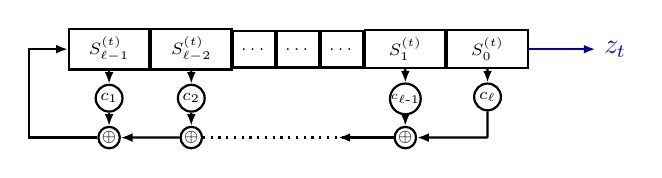
\begin{tikzpicture}[thick, scale=0.85, every node/.style={transform shape}]
        \tikzset{
            regcell/.style={draw, minimum width=1.2cm, minimum height=0.55cm},
            dotcell/.style={draw, minimum width=0.55cm, minimum height=0.55cm},
            multiplier/.style={draw, circle, inner sep=0pt, minimum size=0.4cm, font=\scriptsize},
            xor/.style={draw, circle, inner sep=0pt, minimum size=0.32cm, font=\scriptsize}
        }

        % Register Cells
        \node[regcell] (sL-1) at (0,0) {\scriptsize $S_{\ell-1}^{(t)}$};
        \node[regcell, right=0pt of sL-1] (sL-2) {\scriptsize $S_{\ell-2}^{(t)}$};
        \node[dotcell, right=0pt of sL-2] (dots1) {\scriptsize $\dots$};
        \node[dotcell, right=0pt of dots1] (dots2) {\scriptsize $\dots$};
        \node[dotcell, right=0pt of dots2] (dots3) {\scriptsize $\dots$};
        \node[regcell, right=0pt of dots3] (s1) {\scriptsize $S_{1}^{(t)}$};
        \node[regcell, right=0pt of s1] (s0) {\scriptsize $S_{0}^{(t)}$};

        % Multipliers
        \node[multiplier, below=0.2cm of sL-1] (c1) {$c_1$};
        \node[multiplier, below=0.2cm of sL-2] (c2) {$c_2$};
        \node[multiplier, below=0.2cm of s1] (cL-1) {\tiny $c_{\ell\text{-}1}$};
        \node[multiplier, below=0.2cm of s0] (cL) {$c_\ell$};

        % XOR Gates
        \node[xor, below=0.2cm of c1] (x1) {$\oplus$};
        \node[xor, at={(c2 |- x1)}] (x2) {$\oplus$};
        \node[xor, at={(cL-1 |- x1)}] (xL-1) {$\oplus$};

        \draw[dotted, thick] (x2) -- (xL-1);

        % Connections
        \draw[-{Latex[length=1.5mm]}] (sL-1) -- (c1);
        \draw[-{Latex[length=1.5mm]}] (sL-2) -- (c2);
        \draw[-{Latex[length=1.5mm]}] (s1) -- (cL-1);
        \draw[-{Latex[length=1.5mm]}] (s0) -- (cL);
        \draw[-{Latex[length=1.5mm]}] (c1) -- (x1);
        \draw[-{Latex[length=1.5mm]}] (c2) -- (x2);
        \draw[-{Latex[length=1.5mm]}] (cL-1) -- (xL-1);
        \draw[-] (cL) -- (cL |- x1);
        \draw[-{Latex[length=1.5mm]}] (cL |- x1) -- (xL-1);
        \draw[-{Latex[length=1.5mm]}] (xL-1) -- ++(-1.0,0);
        \draw[-{Latex[length=1.5mm]}] (x2) -- (x1);
        \draw[-{Latex[length=1.5mm]}] (x1) -- ++(-1.2,0) |- (sL-1.west);

        % OUTPUT FROM S0
        \draw[-{Latex[length=1.5mm]}, thick, blue!70!black] (s0.east) -- ++(1.0,0) node[right, font=\large] {$z_t$};
    \end{tikzpicture}
    }
    \end{center}

    \begin{itemize}
        \item \textbf{État} : $S^{(t)} = (S_0^{(t)}, \dots, S_{\ell-1}^{(t)}) \in \mathbb{F}_2^{\ell}$ \hfill (Def. II-4)
        \item \textbf{Mise à jour} : Récurrence linéaire sur $\mathbb{F}_2$.
        \item \textbf{Polynôme de rétroaction} : $f(X) = 1 \oplus c_1 X \oplus \dots \oplus c_{\ell} X^{\ell}$.
        \item \textbf{Période} : $T = 2^{\ell} - 1$ (m-suite, si $f$ primitif). \hfill (Prop. II-5)
    \end{itemize}

    \note{
        - Def. II-4 : LFSR = automate linéaire sur $\mathbb{F}_2$.
        - Prop. II-5 : période max $\iff$ polynôme primitif.
        - Output : $z_t = S_0^{(t)}$ (sortie directe).
        - Hardware efficace, mais structure algébrique transparente.
    }
\end{frame}

% --- SLIDE 2: VULNERABILITY ---
\begin{frame}{La Faiblesse : Berlekamp-Massey}
    \begin{alertblock}{La Linéarité tue la Sécurité}
        Un LFSR brut est régi par des équations linéaires sur $\mathbb{F}_2$. Son polynôme est reconstructible.
    \end{alertblock}

    \vspace{0.2cm}
    \textbf{L'Algorithme de Berlekamp-Massey :}
    \begin{itemize}
        \item Reconstruit le polynôme minimal $f(X)$ d'une suite récurrente linéaire.
        \item Complexité : $\mathcal{O}(\ell^2)$ opérations sur $\mathbb{F}_2$.
        \item Il suffit d'observer \textbf{$2\ell$ bits} consécutifs de la suite chiffrante $z_t$ pour retrouver $S^{(0)}$ et prédire toute la suite.
    \end{itemize}

    \vspace{0.2cm}
    \textit{Pour vendre une machine ``inviolable'', Crypto AG devait briser cette transparence algébrique.}

    \note{
        - Berlekamp-Massey : Thm. II-8.
        - $2\ell$ bits de suite chiffrante $\Rightarrow$ reconstruction complète de $f(X)$ et $S^{(0)}$.
        - LFSR brut $=$ sécurité nulle face à un adversaire compétent.
        - $\Rightarrow$ Nécessité d'introduire de la non-linéarité.
    }
\end{frame}

\begin{frame}{La Solution : Générateur à Combinaison}
    \begin{columns}[c]
        \begin{column}{0.45\textwidth}
            \centering
            \resizebox{\linewidth}{!}{
            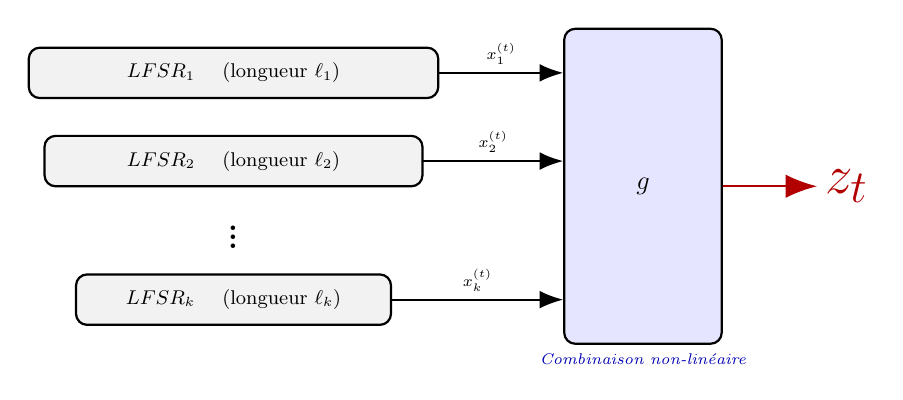
\begin{tikzpicture}[thick, scale=0.8, every node/.style={transform shape}]
                \tikzset{
                    lfsrbox/.style={draw, rounded corners, minimum height=0.8cm, font=\small, align=center, fill=gray!10},
                    gbox/.style={draw, rounded corners, fill=blue!10, minimum width=2.5cm, minimum height=5.0cm, font=\large, align=center}
                }

                \node[lfsrbox, minimum width=6.5cm] (lfsr1) at (0, 2.2)  {$LFSR_1$ \quad (longueur $\ell_1$)};
                \node[lfsrbox, minimum width=6.0cm] (lfsr2) at (0, 0.8)  {$LFSR_2$ \quad (longueur $\ell_2$)};
                \node at (0, -0.3) {\Huge $\vdots$};
                \node[lfsrbox, minimum width=5.0cm] (lfsrk) at (0, -1.4) {$LFSR_k$ \quad (longueur $\ell_k$)};

                \node[gbox] (gbox) at (6.5, 0.4) {$g$};
                \node[below=0.01cm of gbox, font=\scriptsize\itshape, text=blue!70!black] {Combinaison non-linéaire};

                \draw[-{Latex[length=3mm]}, thick] (lfsr1.east) -- node[above, font=\scriptsize, midway] {$x_1^{(t)}$} (lfsr1.east -| gbox.west);
                \draw[-{Latex[length=3mm]}, thick] (lfsr2.east) -- node[above, font=\scriptsize, midway] {$x_2^{(t)}$} (lfsr2.east -| gbox.west);
                \draw[-{Latex[length=3mm]}, thick] (lfsrk.east) -- node[above, font=\scriptsize, midway] {$x_k^{(t)}$} (lfsrk.east -| gbox.west);

                \draw[-{Latex[length=4mm]}, thick, red!70!black] (gbox.east) -- ++(1.5,0) node[right, font=\Huge] {$z_t$};
            \end{tikzpicture}
            }
        \end{column}

        \begin{column}{0.5\textwidth}
            On combine $k$ LFSRs \textbf{indépendants} via une fonction non-linéaire $g$.

            \vspace{0.4cm}
            \begin{block}{Propriétés du Générateur}
                \begin{itemize}
                    \item \textbf{Génération :} $z_t = g(x_1^{(t)}, \dots, x_k^{(t)})$
                    \item \textbf{Période Maximale :} Les $\ell_i$ sont \textbf{premières entre elles}.
                    \item \textbf{Résultat :} $T_{tot} = \prod_{i=1}^k (2^{\ell_i} - 1)$.
                \end{itemize}
            \end{block}
        \end{column}
    \end{columns}

    \note{
        - Réalité industrielle : k entre 3 et 6 LFSRs (ASIC compacts).
        - \textbf{Pourquoi des longueurs différentes ?} Si $\ell_i$ premières entre elles, la période globale est le produit des périodes individuelles (gigantesque pour un coût minime).
        - \textbf{Compromis de Siegenthaler} : Degré algébrique vs Immunité de corrélation.
        - \textbf{Le Leurre} : La NSA a maximisé le degré algébrique de $g$ pour rassurer les ingénieurs.
    }
\end{frame}

\begin{frame}{Minerva : La Backdoor Statistique}
    La NSA conçoit en secret une fonction $g$ \textbf{biaisée} gravée en silicium.
    Le combineur échoue sciemment à satisfaire le critère d'\textbf{immunité de corrélation}.

    \vspace{0.3cm}
    \begin{alertblock}{Le Biais Exploitable}
        Il existe un registre $LFSR_1$ et un biais $\epsilon > 0$ tel que :
        $$P(z_t = x_1^{(t)}) = 0.5 + \epsilon$$
    \end{alertblock}

    \vspace{0.3cm}
    \textbf{Conséquence :} La suite chiffrante $z_t$ ``fuite'' de l'information sur la sortie $x_1^{(t)}$ d'un registre individuel.

    \vspace{0.2cm}
    \textit{Ce biais est invisible à l'usage quotidien, mais statistiquement exploitable avec suffisamment de chiffré.}

    \note{
        - Minerva = violation délibérée de l'immunité de corrélation.
        - \textbf{Astuce NSA} : degré algébrique de $g$ gardé élevé $\Rightarrow$ Berlekamp-Massey reste incalculable $\Rightarrow$ rassure les ingénieurs de Crypto AG.
        - Mais immunité de corrélation sacrifiée $\Rightarrow$ attaque par corrélation possible.
        - Compromis de Siegenthaler exploité à l'envers : la faiblesse est cachée derrière la complexité apparente.
    }
\end{frame}

% ==============================================================================

% 5. ATTACK COMPLEXITY
% ==============================================================================
\section{L'Attaque (Divide \& Conquer)}

\begin{frame}{L'Attaque : \textit{Divide \& Conquer}}
    Le biais $\epsilon$ permet d'attaquer chaque registre $L_i$ \textbf{indépendamment}.

    \vspace{0.3cm}
    \begin{columns}
        \column{0.5\textwidth}
        \begin{center}
            \textbf{Brute Force (sans backdoor)}\\
            \vspace{0.2cm}
            \textcolor{red}{\Large $\mathcal{O}(2^{\sum_{i=1}^k \ell_i})$}\\
            \vspace{0.2cm}
            Espace joint\\
            \textit{Incalculable (siècles).}
        \end{center}

        \column{0.5\textwidth}
        \begin{center}
            \textbf{Corrélation (Minerva)}\\
            \vspace{0.2cm}
            \textcolor{green!60!black}{\Large $\mathcal{O}(\sum_{i=1}^k 2^{\ell_i})$}\\
            \vspace{0.2cm}
            Registres isolés\\
            \textit{Quelques secondes.}
        \end{center}
    \end{columns}

    \vspace{0.4cm}
    \textbf{Méthode :} Avec du \textit{clair probable} (en-tête diplomatique, salutation standard), l'attaquant compare statistiquement chaque état candidat de $L_1$ à la suite chiffrante captée. Le vrai état se démarque par corrélation.

    \note{
        - \textbf{Attaque à clair connu}.
        - Source du clair : en-têtes régulières des télex diplomatiques (``To Mr Ambassador...'').
        - $m_t \oplus c_t = z_t$ $\Rightarrow$ suite chiffrante récupérée.
        - Isoler $LFSR_1$ grâce au biais $\epsilon_1$, soustraire, puis attaquer $LFSR_2$, etc.
        - Exponentielle de la somme $\to$ somme d'exponentielles.
    }
\end{frame}


\begin{frame}[fragile]{Visualisation de l'Attaque en Cascade}
    \begin{center}
    \resizebox{0.85\linewidth}{!}{
    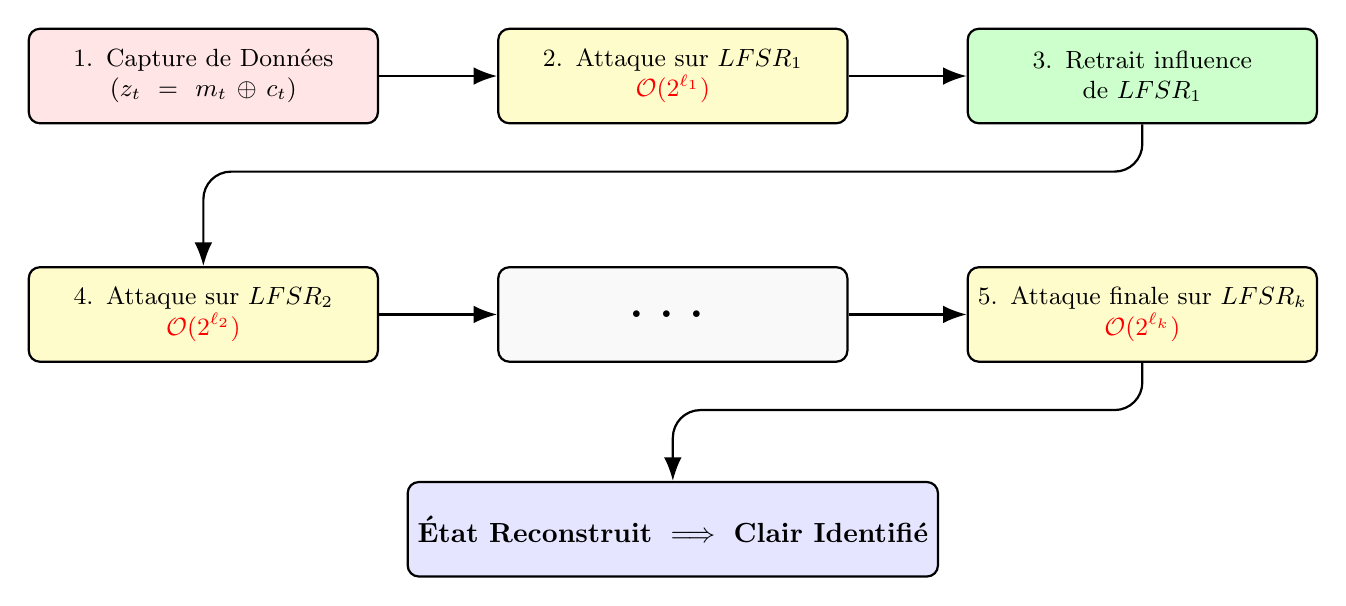
\begin{tikzpicture}[auto, thick, node distance=1.5cm and 1.5cm]
        \tikzset{
            stepnode/.style={draw, rounded corners, align=center, text width=4.2cm, minimum height=1.2cm, font=\small},
            capture/.style={stepnode, fill=red!10},
            attack/.style={stepnode, fill=yellow!20},
            remove/.style={stepnode, fill=green!20},
            finish/.style={stepnode, fill=blue!10, text width=6.5cm, font=\bfseries}
        }

        % --- ROW 1 ---
        \node[capture] (c) {1. Capture de Données\\($z_t = m_t \oplus c_t$)};
        \node[attack, right=of c] (a1) {2. Attaque sur $LFSR_1$\\\textcolor{red}{$\mathcal{O}(2^{\ell_1})$}};
        \node[remove, right=of a1] (r1) {3. Retrait influence\\ de $LFSR_1$};

        % --- ROW 2 ---
        \node[attack, below=1.8cm of c] (a2) {4. Attaque sur $LFSR_2$\\\textcolor{red}{$\mathcal{O}(2^{\ell_2})$}};
        \node[stepnode, fill=gray!5, right=of a2] (dots) {\Huge $\dots$};
        \node[attack, right=of dots] (ak) {5. Attaque finale sur $LFSR_k$\\\textcolor{red}{$\mathcal{O}(2^{\ell_k})$}};

        % --- ROW 3 ---
        \node[finish, below=1.5cm of dots] (f) {État Reconstruit $\implies$ Clair Identifié};

        % Arrows Row 1
        \draw[-{Latex[length=3mm]}] (c) -- (a1);
        \draw[-{Latex[length=3mm]}] (a1) -- (r1);

        % Serpent Connector Row 1 -> Row 2
        \draw[-{Latex[length=3mm]}, rounded corners=10pt] (r1.south) -- ++(0,-0.6) -| (a2.north);

        % Arrows Row 2
        \draw[-{Latex[length=3mm]}] (a2) -- (dots);
        \draw[-{Latex[length=3mm]}] (dots) -- (ak);

        % Serpent Connector Row 2 -> Row 3
        \draw[-{Latex[length=3mm]}, rounded corners=10pt] (ak.south) -- ++(0,-0.6) -| (f.north);

    \end{tikzpicture}
    }
    \end{center}

    \vspace{0.3cm}
    \textbf{Complexité Totale :} $\mathcal{O}(\sum_{i=1}^{k} 2^{\ell_i}) \ll \mathcal{O}(2^{\sum_{i=1}^{k} \ell_i})$

    \note{
        - Attaque itérative : Brise l'exposant (somme des longueurs) en une somme linéaire.
        - Pour k=6, l'attaque prend quelques secondes quand le brute-force prendrait des millénaires.
        - Chaque étape utilise le signal "purifié" de l'influence des registres déjà cassés.
    }
\end{frame}

% ==============================================================================
% 6. LA CHUTE DE L'EMPIRE CRYPTO AG (HANS BÜHLER)
% ==============================================================================
\section{La Chute d'Operation Rubicon}

\begin{frame}{1992 : La Faille Humaine (L'Affaire Hans Bühler)}
    \begin{columns}
        \column{0.6\textwidth}
        \textbf{L'Arrestation en Iran}
        \begin{itemize}
            \item Hans Bühler, ingénieur commercial star de Crypto AG, est brusquement arrêté à Téhéran en 1992.
            \item Le gouvernement Iranien suspecte l'équipement d'être compromis suite à des fuites liées à des assassinats politiques.
        \end{itemize}

        \vspace{0.3cm}
        \textbf{L'Opération Démasquée}
        \begin{itemize}
            \item La CIA et le BND refusent d'intervenir pour protéger la couverture.
            \item Crypto AG finit par payer une étrange rançon/caution de 1\text{M} \$ à l'Iran, puis licencie Bühler.
            \item L'attention médiatique fait s'écrouler le mythe inviolable de la "neutralité suisse".
        \end{itemize}

        \column{0.4\textwidth}
        \begin{center}
            \begin{alertblock}{La Couverture Parfaite}
                Bühler, comme l'immense majorité des ingénieurs suisses de Crypto AG, ignorait totalement la manipulation des schémas d'immunité des LFSR par Minerva !
            \end{alertblock}
        \end{center}
    \end{columns}

    \note{
        Mais alors, si le système était mathématiquement pur en surface, comment l'empire secret Rubicon s'est-il finalement effondré ?

        Ironiquement pour nous analystes d'algorithmes, ce n'est pas un audit cryptographique qui a révélé la faille, mais une grossière erreur humaine ! En 1992, Hans Bühler, un des vendeurs phares de Crypto AG qui vendait ces machines au Moyen-Orient, est brusquement emprisonné par l'Iran. Les iraniens s'étaient rendus compte que l'Ouest anticipait de manière trop miraculeuse leurs frappes terroristes et politiques, et ont logiquement pointé du doigt l'intégrité de ces machines suisses qu'on leur avait lourdement facturées.

        Bühler, qui n'était pas au courant de la fraude, reste emprisonné neuf mois. La CIA a catégoriquement refusé de lever le petit doigt pour ne pas "griller" la couverture technologique. Dès sa libération sous caution, ce traitement injuste le poussera à alerter la presse germanique. De fil en aiguille, les journalistes d'investigation trouveront la relation cachée entre l'usine de Zoug et le BND à Munich. Le secret industriel du siècle venait de s'éteindre.
    }
\end{frame}

\begin{frame}{2020 : La Déclassification et le Washington Post}
    \begin{columns}
        \column{0.55\textwidth}
        \textbf{Le Secret Révélé (\#CRYPTOLEAKS)}
        \begin{itemize}
            \item En Février 2020, une enquête conjointe du \textit{Washington Post} (USA), de la \textit{ZDF} (ALL) et de \textit{SRF} (SUI) dévoile l'entièreté du scandale.
            \item Ils publient des documents de la CIA déclassifiés, prouvant que de 1970 à 1993, la quasi-totalité des communications sécurisées mondiales étaient lues par la NSA.
        \end{itemize}

        \vspace{0.3cm}
        \textbf{Le Coup de Maître}
        \begin{itemize}
            \item Un rapport interne de la CIA décrit l'opération Rubicon comme "Le coup de maître du renseignement du siècle".
        \end{itemize}

        \column{0.45\textwidth}
        \begin{center}
            \includegraphics[height=3.5cm]{images/hagelin.jpg}\\
            \vspace{0.1cm}
            \small \textit{Machine classique Hagelin réputée inviolable.}
        \end{center}
    \end{columns}

    \note{
        Pour conclure définitivement sur ce pan d'histoire, comment a-t-on la certitude absolue de la véracité de cette incroyable opération ?

        En Février 2020 (il y a à peine quelques années), une enquête coup de poing mondiale entre le Washington Post, la télévision allemande et la télévision suisse ont publié ce qu'ils appellent les "Cryptoleaks". Des documents top-secrets de la CIA ont été déclassifiés, et ont formellement prouvé que de 1970 jusqu'à la fin de la guerre froide, ce duo contrôlait plus de 40\% des flux mondiaux cryptés.

        Un rapport interne de l'agence va même jusqu'à qualifier Rubicon de "coup de maître du renseignement du siècle". La société Crypto AG a finalement été liquidée en 2018. Des décennies de communications ultra-secrètes ont été aspirées silencieusement, le tout à cause d'un décalage mathématique subtil sur un polynome de LFSR.
    }
\end{frame}

% ==============================================================================
% 6. REFERENCES (SECOND TO LAST SLIDE)
% ==============================================================================
\section{Références}

\begin{frame}{Références Bibliographiques}
    \begin{itemize}
        \item \textbf{Support de Cours :}
        \begin{itemize}
            \item G. Castagnos, \textit{Cours de Cryptologie 2025-2026}, Univ. Bordeaux.
            \item Chap. II : Chiffrements par flot, LFSR, Berlekamp-Massey, immunité de corrélation.
        \end{itemize}

        \vspace{0.3cm}
        \item \textbf{Sources Historiques \& Techniques :}
        \begin{itemize}
            \item G. Miller, \textit{``The intelligence coup of the century''}, Washington Post, 2020.
            \item T. Pornin, \textit{``The Swiss Cheese of Cryptography''}, SSTIC.
            \item J. Gressel \& CCC, Reverse-Engineering HC-7000, \textit{\#CRYPTOLEAKS}, 2020.
        \end{itemize}
    \end{itemize}
    \note{
        - Fondements mathématiques : Chap. II (Castagnos), Def. II-4, Prop. II-5, Thm. II-8.
        - Source primaire : documents CIA déclassifiés, publiés par le Washington Post.
        - Aspects techniques : reverse-engineering par le CCC (Leipzig 2020).
    }
\end{frame}

% ==============================================================================
% 7. CONCLUSION
% ==============================================================================
\section{Conclusion}

\begin{frame}
    \centering
    \Huge \textbf{Questions ?}

    \vspace{1cm}
    \normalsize
    \textit{``Trust, but Verify.''}\\
    \vspace{0.2cm}
    \small -- \textbf{Ronald Reagan}, sommets nucléaires (1987)
    
    \vspace{0.5cm}
    \normalsize
    \textit{Ou plutôt : ``Don't trust. Open-Source everything.''}

    \note{
        - L'Opération Rubicon est la preuve définitive que ``Security by Obscurity'' est une faille.
        - Confier des communications étatiques à du hardware propriétaire non-audité $=$ backdoor garantie.
        - La leçon : seuls les algorithmes publics (AES, standards NIST) audités par la communauté offrent une sécurité réelle.
        - Merci. Questions bienvenues sur les LFSR, la corrélation, ou le contexte géopolitique.
    }
\end{frame}

\end{document}